%<dscrpt>Equation differentielle linéaire du premier ordre et tangentes.</dscrpt>
\begin{figure}[!ht]
 \centering
 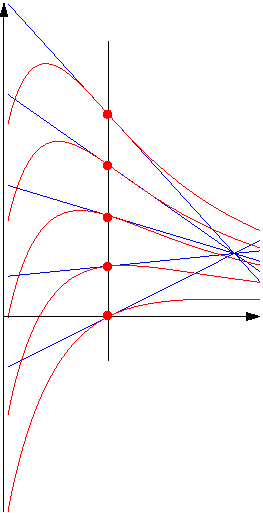
\includegraphics{Eeqd7_1.pdf}
 % Eeqd7_1.pdf: 0x0 pixel, 0dpi, nanxnan cm, bb=
 \caption{Des tangentes aux graphes de solutions}
 \label{fig:Eeqd7_1}
\end{figure}

On rappelle que si $f$ est une fonction définie dans un intervalle de $\R$ et à valeurs réelles, l'équation de la tangente en un point $(x_0,f(x_0))$ à la courbe représentative de $f$ s'écrit :
\[
\begin{array}{|cc|}
 x-x_0 & 1  \\ 
 y-f(x_0)& f'(x_0) 
\end{array}=0
\]
On considère l'équation differentielle\footnote{d'après un problème de Serge Dupont (\href{http://moduloserge.free.fr/}{http://moduloserge.free.fr/}) } dans $I=]0,+\infty[$
\begin{equation}
(1+x^2)y'(x)+2xy(x)=\frac{1}{x} \label{Eeqd7:1}
\end{equation}
\begin{enumerate}
\item Soit $f$ une solution de (\ref{Eeqd7:1}), on pose $\lambda=f(1)$.
\begin{enumerate}
\item Former l'équation de la tangente en $(1,\lambda)$ à la courbe de $f$.
\item Montrer que lorsque $\lambda$ varie, ces tangentes sont toutes concourantes en un point à déterminer.
\end{enumerate}
\item Résoudre l'équation (\ref{Eeqd7:1}) sur $I$. Déterminer l'unique solution $f_\lambda$ telle que $f_\lambda(1)=\lambda$.
\item Soit $I$ un intervalle de $\R$ et $a$, $b$, $c$ trois fonctions continues définies dans $I$. On suppose que $a$ ne prend jamais la valeur 0.
On considère l'équation
\begin{equation}
ay'+by=c \label{Eeqd7:2}
\end{equation}
Soit $x_0\in I$ fixé, pour tout $\lambda$ réel, on note $f_\lambda$ la solution de (\ref{Eeqd7:2}) qui prend en $x_0$ la valeur $\lambda$. On note $\mathcal{D}_\lambda$ la tangente en $(x_0,\lambda)$ à la courbe de $f_\lambda$.
Montrer que les droites $\mathcal{D}_\lambda$ sont concourantes ou parallèles. Préciser dans quel cas elles sont parallèles. Lorsqu'elles sont concourantes préciser leur point commun.

\item Soient $J$ un intervalle de $\mathbb{R}$ et $F$ une fonction de $J\times\mathbb{R}$ dan s$\R$. Notons $(E)$ l'équation différentielle
\begin{displaymath}
y'=F(x,y)\qquad (E) 
\end{displaymath}
On suppose que $F$ est telle que:
  \begin{itemize}
\item pour tout $(x_0,y_0)\in J\times \R$, il existe une solution de $(E)$ satisfaisant la condition de Cauchy $y(x_0)=y_0$;
\item les tangentes au point d'abscisse $x_0$ aux solutions de $(E)$ sont soit toutes parallèles, soit toutes concourantes.
  \end{itemize}
  \begin{enumerate}
    \item Pour $x_0\in J$ et $(y_0,y_1)\in\R^2$ avec $y_0\neq y_1$, montrer que 
\begin{displaymath}
\frac{F(x_0,y_0)-F(x_0,y_1)}{y_0-y_1} 
\end{displaymath}
est une quantité qui ne dépend pas du couple $(y_0,y_1)$. On la notera $\alpha(x_0)$ dans la suite .
    \item En déduire que $F(x_0,y_0)-\alpha(x_0)y_0$ ne dépend pas de $y_0$.
    \item Conclure que $(E)$ est linéaire c'est-à-dire que $F$ est de la forme $F(x,y)=\alpha(x)\cdot y+\beta(x)$ , pour $(x,y)\in J\times \R$ avec $\alpha$ et $\beta$ deux fonctions.
  \end{enumerate}

\end{enumerate}
